\documentclass{standalone}
\usepackage{graphicx}	
\usepackage{amssymb, amsmath, amsthm}
\usepackage{color}

\usepackage{tikz}
\usetikzlibrary{math, calc, arrows.meta}

\definecolor{light}{RGB}{220, 188, 188}
\definecolor{mid}{RGB}{185, 124, 124}
\definecolor{dark}{RGB}{143, 39, 39}
\definecolor{highlight}{RGB}{180, 31, 180}
\definecolor{gray10}{gray}{0.1}
\definecolor{gray20}{gray}{0.2}
\definecolor{gray30}{gray}{0.3}
\definecolor{gray40}{gray}{0.4}
\definecolor{gray60}{gray}{0.6}
\definecolor{gray70}{gray}{0.7}
\definecolor{gray80}{gray}{0.8}
\definecolor{gray90}{gray}{0.9}
\definecolor{gray95}{gray}{0.95}
  
\begin{document}

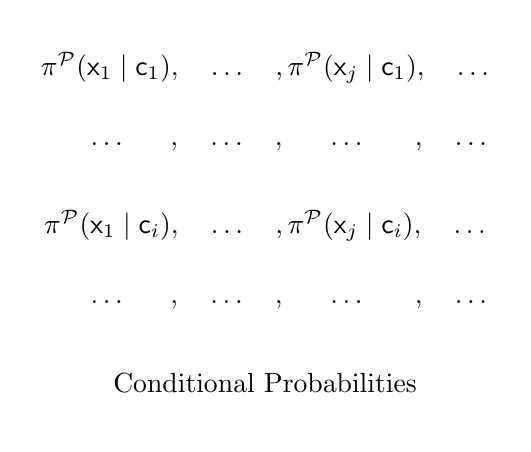
\begin{tikzpicture}[scale=1, thick]

  \pgfmathsetmacro{\dy}{0}
  \begin{scope}[shift={(0, \dy)}]
    \draw[white] (-3, -0.5) rectangle (3, 0.5);
    \node at (0, 0) { $\pi^{\mathcal{P}}(\mathsf{x}_{1} \mid \mathsf{c}_{1}),
                       \quad \ldots \quad,
                       \pi^{\mathcal{P}}(\mathsf{x}_{j} \mid \mathsf{c}_{1}),
                       \quad \ldots$ };
  \end{scope}
  
  \pgfmathsetmacro{\dy}{-1}
  \begin{scope}[shift={(0, \dy)}]
      \draw[white] (-3, -0.5) rectangle (3, 0.5);
      \node at (0, 0) { $\quad\;\;\, \ldots \quad\;\;, \quad \ldots \quad, \;\;\quad \ldots \quad\;\;\,, \quad \ldots$ };
  \end{scope}
  
  \pgfmathsetmacro{\dy}{-2}
  \begin{scope}[shift={(0, \dy)}]
    \draw[white] (-3, -0.5) rectangle (3, 0.5);
    \node at (0, 0) { $\pi^{\mathcal{P}}(\mathsf{x}_{1} \mid \mathsf{c}_{i}),
                       \quad \ldots \quad,
                       \pi^{\mathcal{P}}(\mathsf{x}_{j} \mid \mathsf{c}_{i}),
                       \quad \ldots$ };
  \end{scope}
  
  \pgfmathsetmacro{\dy}{-3}
  \begin{scope}[shift={(0, \dy)}]
      \draw[white] (-3, -0.5) rectangle (3, 0.5);
      \node at (0, 0) { $\quad\;\;\, \ldots \quad\;\;, \quad \ldots \quad, \;\;\quad \ldots \quad\;\;\,, \quad \ldots$ };
  \end{scope}

  \begin{scope}[shift={(0, -4)}]
    \draw[white] (-3, -0.5) rectangle (3, 0.5);
    \node at (0, 0) { Conditional Probabilities };
  \end{scope}

\end{tikzpicture}

\end{document}  